\documentclass{standalone}
\usepackage{tikz}
\usepackage{pgfplots}
\usetikzlibrary{arrows.meta}

\begin{document}

\resizebox{8cm}{8cm}{%
    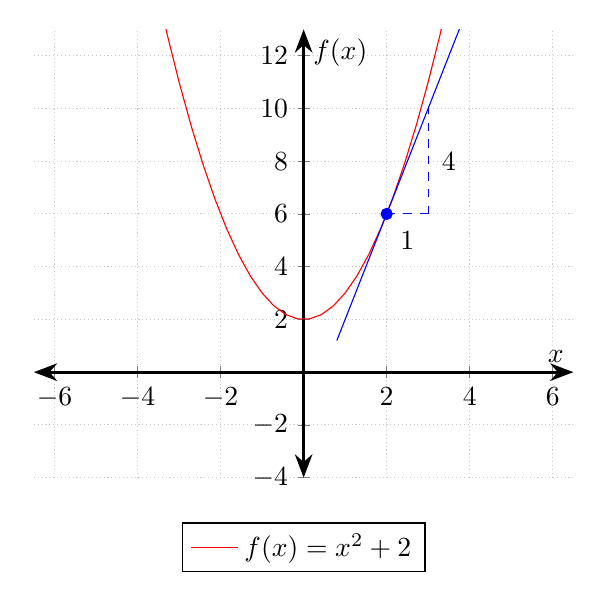
\begin{tikzpicture}
    \begin{axis}[
        title={},
        axis lines=middle,
        axis line style={Stealth-Stealth,very thick},
        xlabel=$x$,
        ylabel={$f(x)$},
        xmin=-6.5,xmax=6.5,ymin=-4,ymax=13,
        xtick distance=2,
        ytick distance=2,
        grid=major,
        grid style={thin,densely dotted,black!20},
        % Bottom center
        legend style={
            at={(0.5,-0.1)},
            anchor=north,
            cells={anchor=west}
        }
    ]
    \addplot[
        domain= -7:7,
        samples=50,
        color=red
        ]
        {x^2+2};
    % Add tangent line at x = 2
    \addplot[
        domain= .8:7,
        samples=50,
        color=blue
        ]
        {4*x-2};
    % Add dot at (2,6)
    \addplot[
        color=blue,
        mark=*,
        only marks,
        mark options={color=blue}
        ]
        coordinates {
            (2,6)
        };
    % dashed line from (2,6) to (3,6) and label 1 under line
    \addplot[
        color=blue,
        mark=none,
        dashed
        ]
        coordinates {
            (2,6)
            (3,6)
        };
    \node at (axis cs:2.5,5) {1};
    % dashed line from (3,6) to (3,10) and label 4 to the right of line
    \addplot[
        color=blue,
        mark=none,
        dashed
        ]
        coordinates {
            (3,6)
            (3,10)
        };
    \node at (axis cs:3.5,8) {4};
    \addlegendentry{$f(x) = x^2+2$}
    \end{axis}
    \end{tikzpicture}
}

\end{document}
